\mysection{The Murk}{species-murk}

  \flavor{Once the gods walked upon Earth as men walk and spake with their mouths like Men. That was in Wornath-Mavai ... a garden fairer than all the gardens upon Earth. Kib was propitious, and Mung raised not his hand against it, neither did Sish assail it with his hours... \\~ \Tilde Lord Dunsany, \myital{The Gods of Pegana}}


\begin{center}
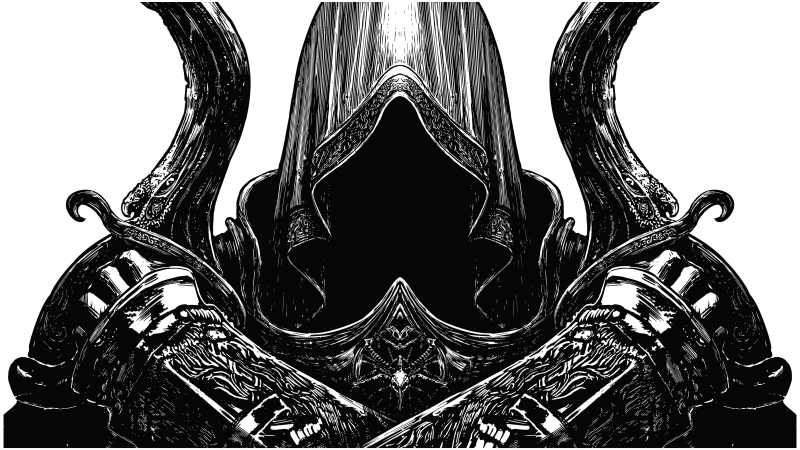
\includegraphics[scale=.45,keepaspectratio=true]{species/Murk2}
\end{center}


\mysubsection{Creation}{murk-creation}

  Write down the following information on your \mylink{Adventurer Sheet}{adventurer-sheet.7}
  
  \callout {
    \mynumlist {
        \item You start with \mybold{4 Flesh and 6 Grit}.
        \item Move your \CLR \DCUP (to a d6).
        \item If you need to \RSTRY{\CLR}, you only fail on a natural 1 (instead of a 1 or 2). Put a check next to \CLR on your Adventurer Sheet so you don't forget.
        \item Choose the empire you have been \mylink{Emancipated}{murk-emancipated} from (see below).
        \item Write down your \mylink{Virtues}{murk-virtues}.
        \item Write down your \mylink{Complication}{murk-complications}.
        \item Write down your \mylink{Starting Gear}{murk-starting-gear}.
    }
 }


\newpage

\begin{multicols*}{2}\raggedcolumns


  \mysubsection{Appearance}{murk-appearance}

  Wornath-Mavai. Svartalfheim. The Glorious Undergarden, beauty beyond measure, Paradise beneath the Mountains, Home to the \Murk, the people beyond Time, who live only for the now.

  Like your brothers and sisters the Spriggan, you were cursed with curiosity, and wondered what was outside of Svartalfheim.  Further and further did you adventure beyond the borders of Svartalfheim until, one day, you were unable to find your way back.  You are now one of the Nomadic People, the Rom.

  Outside of Svartalfheim you were almost immediately enslaved by one of the underworld Empires, for they take great delight in subjugating gods to work for them.  But the burning desire to be free never left you. Almost all \Murk attempt to escape their masters.  Most are killed trying to escape, ending their torment, but some make it out and make their way to the surface.  

  \Murk often act as guides in the Veins, and as such many Mortal races feel that "Murks" are desperate to find their way back again. But the truth is that you can't go back to the point before you knew of the world outside of Svartalfheim.  You have eaten from the tree of knowledge and have been cast out of Eden.  You can never go home again.

  You are tall and thin - like your overworld brethren the Spriggan - but a little shorter, standing less than 2m tall.  Your face resembles Mortals though your eyes and pupils are of the same color: usually cobalt, white, or ruby.  You seem to care little for fashion, yet you are always effortlessly well-dressed in black, white, or gray.  Masks are common among Murks - their captors often heavily scar their faces and bodies out of envy of their beauty - as are broken manacles and collars.

\myimage{species/Murk1}

  \mysubsection{The Veins of the Earth}{murk-veins-of-the-earth}

\ed{The Veins of the Earth, as they are collectively known, have adventures and rules all their own.  Patrick Stuart's excellent \href{http://www.lotfp.com/store/index.php?route=product/product&product_id=262}{"Veins of the Earth"} is the sourcebook used by The Totality of Ygg.}

  According to those who have dared to set foot beneath the skin of the planets of the Totality, the deep places of the moons are beyond description.  They are realms of wondrous colors, breathtaking landscapes, powerful magic, and boundless plenty.  It is a paradise beneath our feet.  The Empires that dwell within stagger the breadth and depth of the surface realms; they shape the caverns and tunnels according to their will, blessed by a deity some heretics say is older than \TheAuthority.  They are truly the gods' people.  You, however, will never meet one - the denizens do not leave their home, save for the unlucky and foolish \Murk.  Why would they?  There is nothing in the world without that the depths cannot provide. Those fortunate explorers who are able to discover an entrance to the depths never return - only a fool turns his back on paradise flowing through the \mylink{Veins of the Earth}{atlas-veins-earth}.


  \myhighlight{Emancipated}{murk-emancipated}

  You are an escaped slave from one of the Empires of the \mylink{Veins of the Earth}{atlas-veins-earth}.  You care for nothing but freedom.  

  Many Mortals find you alien, cold, and uncaring.  This is because \TheAuthority has stolen their freedom from them - the freedom to ask questions, the freedom to go where you desire and do what you wish.  You will never allow your freedom to be taken again, and you will kill to defend both your freedom and the freedom of others.


\callout{\footnotesize{

  You are a renegade from the following Empire (Choose, or roll a d4):
  
   \myskip

    \mybold{Deep Janeen:}   You've worked the mazes and artworks of the Janeen.  If you are underground, you cannot get lost. You are Trained (d8,+1) in the \mylink{Skill: Veins Lore}{skill-veins-lore}. The Janeen only keep the most beautiful and interesting slaves - move your \PRE \DCUP. 

      \myskip

     \mybold{\AelfAdal} The never ending hate of the {\fontfamily{lmtt}\fontseries{b}\selectfont \bfseries{Ælf-Adal}} has burned out your empathy.  You cannot become \mylink{Disgusted}{effect-disgusted} or \mylink{Enraged}{effect-enraged}. If you ever need to try your \INSANITY, you only fail on a 1 (put a checkmark next to \INSANITY on your Adventurer Sheet so you don't forget).

      \myskip

     \mybold{Dvargir:}   You have participated in The Work, and now The Work is part of you.  You never tire and do not need to sleep unless you desire it (you must still rest in order to heal your wounds). You can carry +4 \mylink{Burden}{gear-burden}. Move your \TAL \DCUP.

      \myskip

     \mybold{dErO:}   You possess a partial congruity knot in your skull.  You cannot be \mylink{Befuddled}{effect-befuddled}, \mylink{Charmed}{effect-charmed} or \mylink{Slept}{effect-slept} against your will. You've got experience with dErO "machines" - you are Trained (d8,+1) in \mylink{Skill: Tinkering}{skill-tinkering}.

}}

\cbreak

  \mysubsection{Virtues}{murk-virtues}

  \myhighlight{Child of Gloom}{murk-virtue-child-gloom}

  You have lived your life in the darkness of the Veins, giving you \mylink{Darksight}{effect-darksight}.


  \myhighlight{Fate's Hand}{murk-virtue-fates-hand}

  The Fates smile upon you. Your \INJURY starts at Solid (d4) and your \INSANITY starts at Sober (d4). 


   \myhighlight{Killer}{murk-virtue-killer}

    Provided you get \mylink{the Drop}{combat-drop} on somebody with a weapon forged in \mylink{the Veins of the Earth}{atlas-veins-earth}, you may execute a \mylink{Murder}{vulgate-whispers-murder}. See the section on \mylink{Whispers of the Bride}{vulgate-whisper-the-bride} for more details.

  \myhighlight{Metal Empathy}{murk-virtue-metal-empathy}

  You can smell any type of metal (and the type of metal it is) up to 1 meter away. You can detect if a metal object is Magic or not by touch.

  \myhighlight{Silent Speech}{murk-virtue-silent-speech}

  You know the \mylink{Silent Speech}{atlas-languages}, the language of stones and rocks and the trade speech of the \mylink{Veins of the Earth}{atlas-veins-earth}.  You can use this language to speak with stones. They can tell you what has touched them and what is under or behind them.  This makes it almost impossible to get lost underground. They're not great with time though ...

  \myhighlight{Undreamt}{murk-virtue-undreamt}

  You stand outside of the Dream and are thus untouched by Sish, the Handmaiden of Time. You are immune to aging of any kind, and your \DEATH starts at Tough (d4).

\newpage

  \mysubsection{Complications}{murk-complications}


  \myhighlight{Alien}{murk-complication-alien}

  As far as Mortals are concerned, you are deeply and fundamentally \myital{weird}. You are eerie and alien, and it's not uncommon for other creatures to react to your presence with fear or loathing. Dogs bark at your approach, a cold breeze seems to follow you, you don't blink enough and your smile never seems to touch your eyes. You are one of the Rom, the Nomadic People - and there are no campfires where you will find welcome, save with your Band.



  \myhighlight{Sun Allergy}{murk-complication-sun-allergy}

  Prolonged exposure to direct sunlight causes severe burns and painful blisters.  You seek out shade and shadow whenever you can, and you are most comfortable in subterranean settings.  You can travel well enough through wooded or hilly areas, but wide exposure (deserts, plains) can be problematic if you don't take precautions (Arbiter's discretion).

  \myhighlight{Unseelie}{murk-complication-unseelie}
    
  You are creature of Chaos, one of the \mylink{Unseelie}{the-inhabitants} - and are thus \mybold{Unhallowed}.

\cbreak


  \mysubsection{Starting Gear}{murk-starting-gear}

  \callout{\footnotesize{
  You begin with:

      \mybullet {
        \item a suit of \mylink{Light Armor}{gear-armor};
        \item two insect mandibles (treat as a \mylink{Short Swords}{gear-dex-weapons}) or a Knotsman \mylink{War Axe}{gear-vig-weapons} (these weapons are considered to have been forged in the \mylink{Veins of the Earth}{atlas-veins-earth})
        \item \UDD{d4} of \mylink{Personal Provisions}{gear-equipment};
        \item 2 pet rocks (tell the Arbiter their names);
        \item a journal filled with names and locations that lead nowhere;
        \item a leather folio of maps that lead nowhere;
        \item a pouch of 50 tokens used by the slaves in the culture you've escaped from;
        \item a pouch of 5 gems (roll on the \mylink{Gems table}{appendix-a-gems} in Appendix A).

      }}}


    \myhighlight{What Next?}{murk-what-next}

    Be sure you understand how \mylink{the Drop}{combat-drop} (see \mylink{Fighting}{combat-fighting} under \mylink{Combat}{combat}) and \mylink{Murder}{vulgate-whispers-murder} work (details in the section on \mylink{Whispers of The Bride}{vulgate-whisper-the-bride}), and read up on the \mylink{Veins of the Earth}{atlas-veins-earth}.

\end{multicols*}

